\documentclass[a4paper,12pt]{article}
\usepackage[utf8]{inputenc}
\usepackage[magyar]{babel}
\usepackage[T1]{fontenc}
\usepackage{graphicx}
\usepackage{geometry}
\usepackage{hyperref}
\usepackage{listings}
\usepackage{xcolor}
\usepackage{float}
\usepackage{enumitem}
\usepackage{titlesec}

% Margók beállítása
\geometry{left=2.5cm, right=2.5cm, top=2.5cm, bottom=2.5cm}

% Szakasz címek formázása
\titleformat{\section}{\Large\bfseries}{\thesection}{1em}{}
\titleformat{\subsection}{\large\bfseries}{\thesubsection}{1em}{}
\titlespacing*{\section}{0pt}{1.5em}{0.8em}
\titlespacing*{\subsection}{0pt}{1.2em}{0.6em}

% Hivatkozások stílusa
\hypersetup{
    colorlinks=true,
    linkcolor=blue,
    urlcolor=blue
}

% Kódblokk stílusok
\definecolor{codegray}{rgb}{0.95,0.95,0.95}
\definecolor{codeblue}{rgb}{0.1,0.1,0.6}
\definecolor{codegreen}{rgb}{0.1,0.4,0.1}

\lstdefinestyle{pythonstyle}{
    backgroundcolor=\color{codegray},
    commentstyle=\color{codegreen},
    keywordstyle=\color{codeblue}\bfseries,
    numberstyle=\tiny\color{gray},
    stringstyle=\color{red!60!black},
    basicstyle=\ttfamily\footnotesize,
    breaklines=true,
    captionpos=b,
    keepspaces=true,
    frame=single,
    showstringspaces=false,
    language=Python
}
\lstset{style=pythonstyle}

\title{\textbf{Beadandó Dokumentáció}\\ \large AI Code Auditor – Intelligens Kódelemző Platform}
\author{Hasznos Norbert Bendegúz \\ \small DN04PZ}
\date{\today}

\begin{document}

\maketitle

\vspace{1em}

\section{Feladat azonosítója és címe}

\noindent
\begin{tabular}{@{}ll}
\textbf{Azonosító:} & A34 \\
\textbf{Cím:} & \textit{LLM alapú kódelemző rendszer} – LLM alapú, automatizált \\
& kódminőség-ellenőrző és biztonsági auditor webalkalmazás fejlesztése.
\end{tabular}

\section{A feladat megoldásának körülményei}

A modern szoftverfejlesztésben a kódátvizsgálás (code review) kritikus, de időigényes folyamat. A projekt célja egy olyan grafikus felülettel rendelkező eszköz létrehozása volt, amely képes kiváltani a manuális review első körét, azonnali visszajelzést adva a fejlesztőnek a biztonsági résekről, teljesítménybeli problémákról és a kódminőségről.

A megoldáshoz a \textbf{Python} nyelvet és a \textbf{Streamlit} keretrendszert választottam, mivel ezek teszik lehetővé a leggyorsabb prototípuskészítést adatvezérelt alkalmazásokhoz. A "motorháztető alatt" a rendszer két vezető AI modellt támogat: az \textbf{OpenAI GPT-4o}-t a mélyebb elemzésekhez és a \textbf{Google Gemini}-t a költséghatékonyabb működéshez. Kiemelt figyelmet fordítottam a felhasználói élményre (Dark Mode, reszponzív UI) és a hordozhatóságra, ezért az alkalmazás teljeskörűen \textbf{Dockerizálva} lett.

A fejlesztés során sikerült megvalósítani egy robusztus rendszert, amely nemcsak elemzi a kódot, hanem vizuális statisztikákat (Plotly diagramok) is készít, valamint lehetőséget ad az eredmények PDF, JSON vagy Markdown formátumú exportálására. A \textit{Batch Analysis} funkcióval teljes projektek átvizsgálása is megoldott.

\begin{figure}[H]
    \centering
    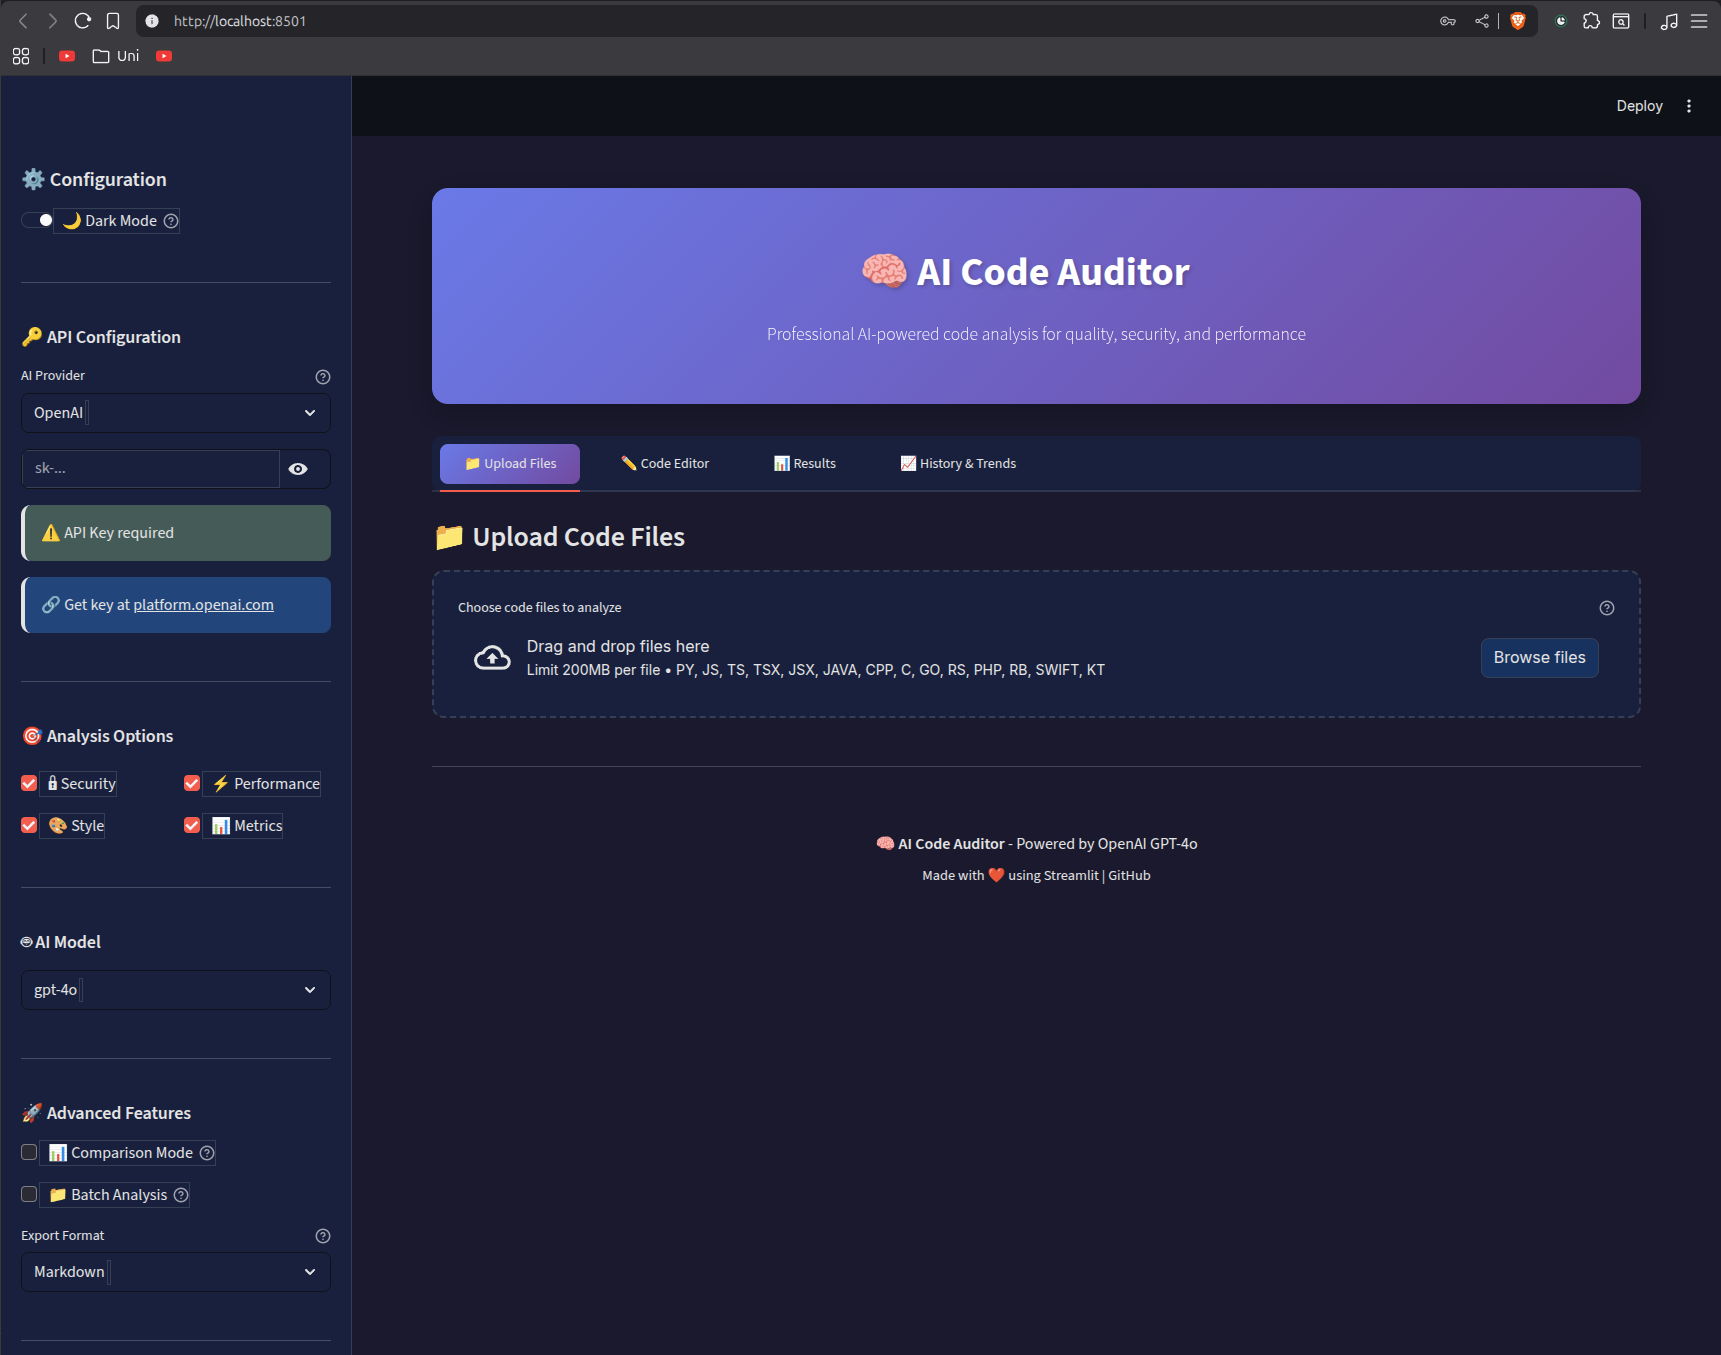
\includegraphics[width=0.85\textwidth]{images/main-page.png} 
    \caption{Az AI Code Auditor főképernyője.}
    \label{fig:main-page}
\end{figure}

\section{A feladat megoldása}

A projekt teljes forráskódja, beleértve a Docker konfigurációt és a részletes telepítési útmutatót, elérhető a GitHub repository-ban.

\noindent \textbf{Git Repository:} \url{https://github.com/Fustli/ai-code-auditor}

\subsection*{Architektúra és Prompt Engineering}
Az alkalmazás szíve a \texttt{src/code\_analyzer.py} modul, amely a felhasználó által feltöltött fájlokat és a kiválasztott beállításokat (pl. Security Focus, Performance Check) egy komplex prompttá alakítja.

A megoldás során kulcsfontosságú volt a \textbf{strukturált kimenet} kikényszerítése az LLM-től, hogy a Streamlit felületén szép táblázatokat és grafikonokat tudjak megjeleníteni a nyers szöveg helyett.

\vspace{0.5em}

\newpage

\begin{lstlisting}[caption=Részlet a rendszer által használt prompt logikából]
SYSTEM_INSTRUCTION = """
You are AI Code Auditor, an expert software architect.
Analyze the code based on the following weights:
- Code Quality: 40% (Readability, DRY, SOLID)
- Security: 35% (OWASP Top 10, Injection flaws)
- Performance: 25% (Complexity, Resource usage)

Output Format: Strictly valid JSON with specific keys:
"score", "grade" (A-F), "issues" (list with severity), "recommendations".
"""
\end{lstlisting}

\vspace{0.5em}

A rendszer \texttt{pydantic} alapú validációt használ, hogy biztosítsa: a kapott válasz mindig feldolgozható formátumú. A frontend oldalon a \texttt{Streamlit-Ace} komponenst használtam a szintaxis-kiemelt kódszerkesztéshez, a diagramokért pedig a \texttt{Plotly} felel.

\begin{figure}[H]
    \centering
    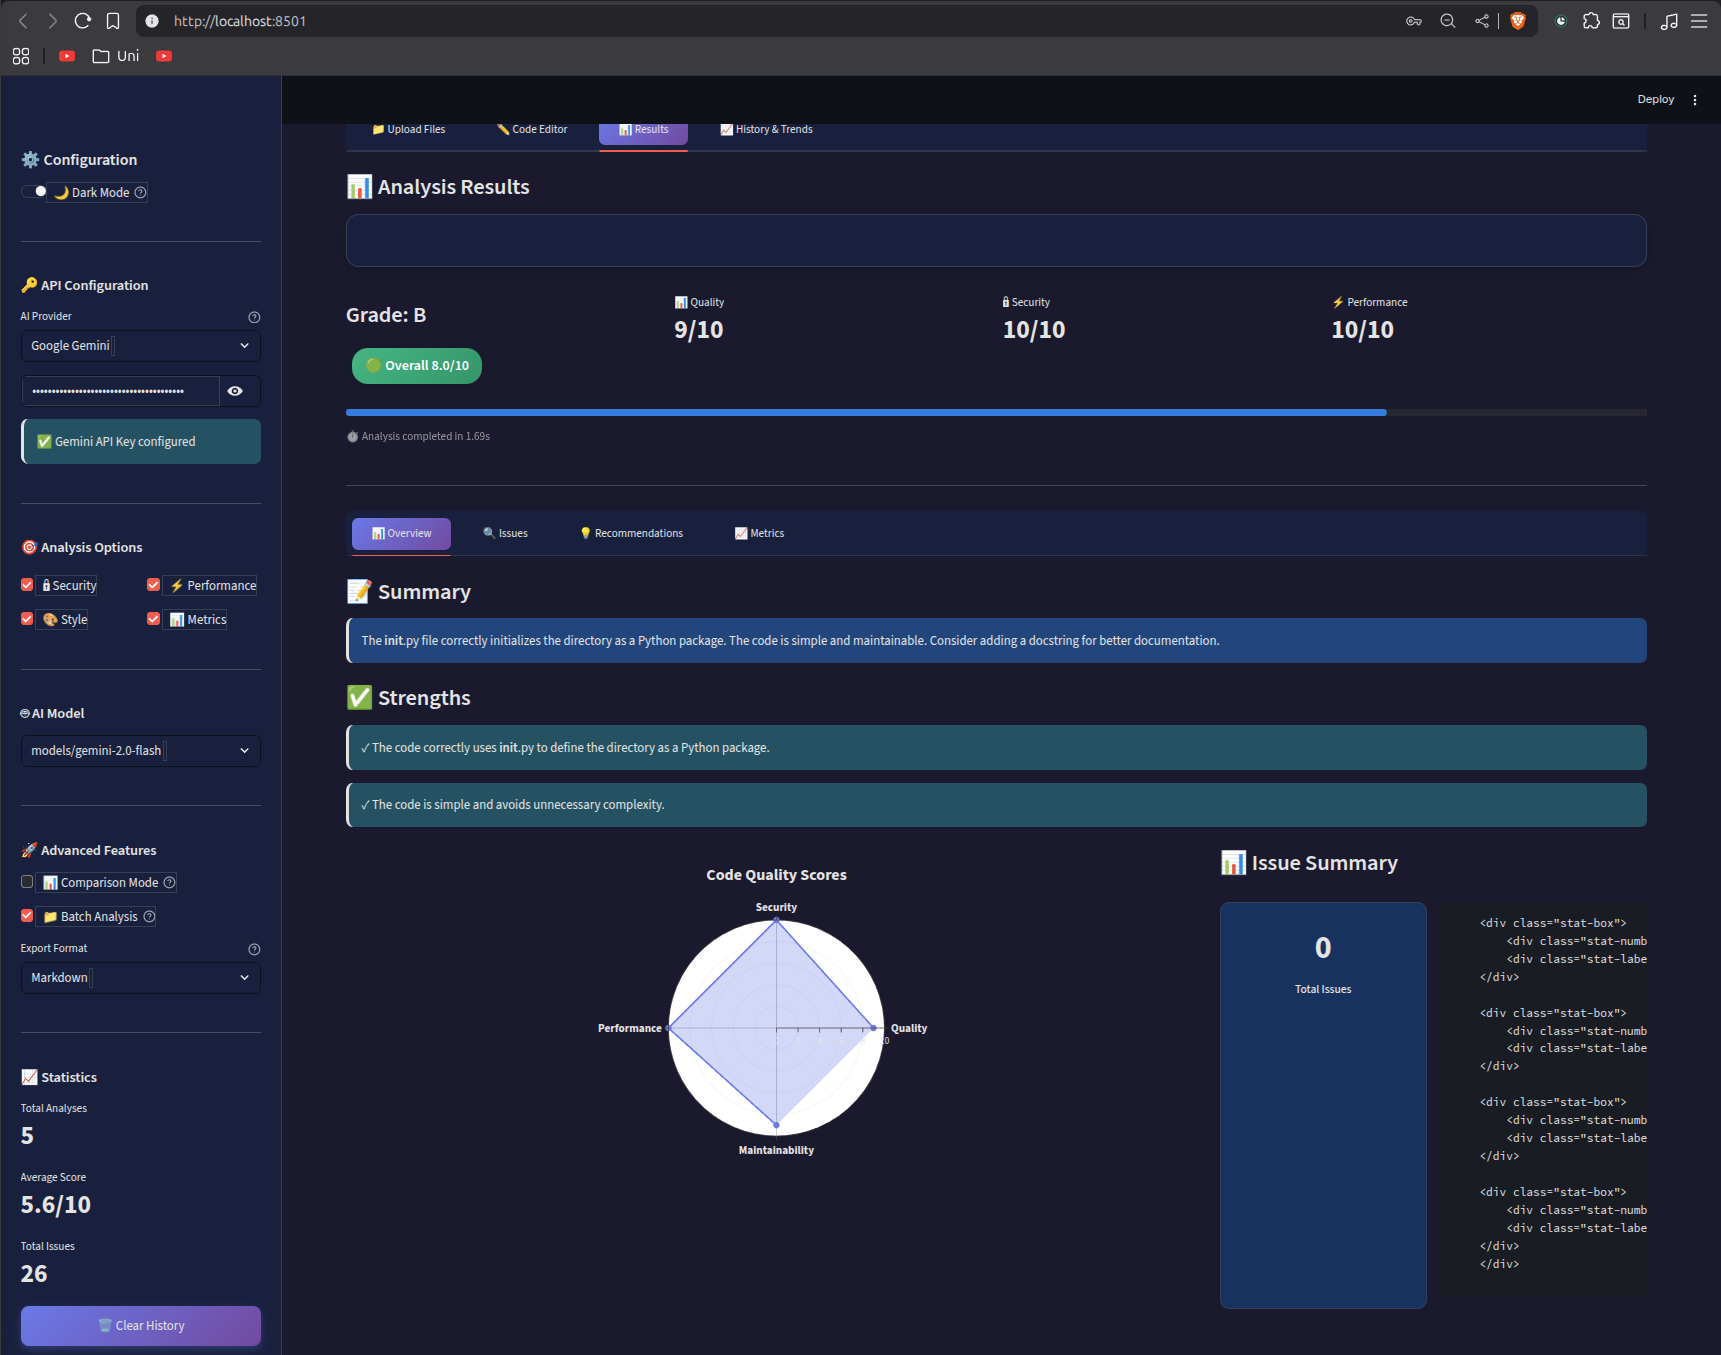
\includegraphics[width=0.85\textwidth]{images/overview.png}
    \caption{Elemzési eredmények: Radar diagram a kódminőségről}
    \label{fig:overview}
\end{figure}

\vspace{1em}

\section{Szakmai tanulságok: Prompt Engineering}

A projekt legértékesebb hozadéka a modern Prompt Engineering technikák gyakorlati elsajátítása volt. Rájöttem, hogy az "utasítsd az AI-t" megközelítés helyett strukturált mérnöki módszerekre van szükség a megbízható működéshez.

\subsection*{1. Context Provisioning (Kontextus biztosítása)}
Megtanultam, hogy az LLM nem látja a "nagy képet", hacsak nem adjuk meg neki explicit módon. Nem elég csak a kódot beküldeni; a "Context Provisioning" során metadatokat (fájlnév, programozási nyelv, kapcsolódó config fájlok) is csatoltam a prompt-hoz. Ez drasztikusan csökkentette a tévesztéseket (pl. nem keverte össze a Java és JavaScript szintaxist hasonló kódrészleteknél).

\vspace{0.5em}

\subsection*{2. Role-Based Prompting (Szerepkör alapú utasítás)}
A tesztek során kiderült, hogy ha nem definiálok "személyiséget", a válaszok túl általánosak. A "Role-Based Prompting" alkalmazásával (pl. \textit{"You are a Senior Security Engineer specialized in OWASP vulnerabilities..."}) a modell "hangszíne" megváltozott: sokkal kritikusabb, technikaibb és precízebb hibákat tárt fel, mintha csak azt írtam volna, hogy "Check this code".

\vspace{0.5em}

\subsection*{3. Chain of Thought (Gondolatmenet-lánc)}
A komplexebb logikai hibák megtalálásához bevezettem a "Chain of Thought (CoT)" technikát. Ahelyett, hogy azonnal a végeredményt kértem volna, arra utasítottam a modellt, hogy lépésről lépésre elemezze a kódot (pl. "First, analyze the data flow, then check for input validation..."). Ez a módszer segített feltárni olyan rejtett hibákat (pl. race condition), amiket a "zero-shot" kérések gyakran kihagytak.

\vspace{0.5em}

\subsection*{4. Few-Shot Learning (Példa alapú tanulás)}
A legnagyobb technikai kihívást a strukturált (JSON) kimenet garantálása jelentette a Streamlit UI számára. Itt a "Few-Shot Learning" bizonyult megoldásnak: a promptba beágyaztam 2-3 példát (bemenet -> elvárt JSON kimenet). Ezután a modell már 99\%-os pontossággal tartotta be a kért sémát, így a backend hibamentesen tudta feldolgozni a választ.

\end{document}

